\section{Introduction}
\label{sec:intro}

The study of detecting and quantifying human emotion has been a topic for many years. Going back to 1894, William James proclaimed that emotion is a result of our actions \cite{james1948emotion}. More important though was his idea that emotion correlates to feeling \cite{james2007principles}. Emotions themselves are induced by stimuli, which excite the human subject and thus propagates to bodily change. According to Izard, the core theories that view cognitive and sensory processes as emotional activators can be followed back to James \cite{izard1990substrates}.

Going forward several years into the mid-90s, Picard consolidated ideas of computing and measuring affect in her 1995 essay, coining the term Affective Computing \cite{picard2000affective}. A subfield of affective computing is based around recognising affective states from facial expressions. Much of the progress in this field bases its research around several axiomatic assumptions, one of which being that all facial movements are induced by emotion. This is especially problematic if the analysed subject is speaking, since the act of talking also triggers facial movement and thus introduces noise into the input data. 

In this thesis, we want to find ways to make existing facial expression recognition models more robust towards talking subjects. We will analyse how humans detect emotion when confronted with speaking people (Chapter \ref{sec:human}), and try to include those findings in our models (Chapter \ref{sec:models}). We further benchmark our models against inputs of different languages, and speech acts that are more akin to those in the real world (Chapter \ref{sec:data}).

We conclude our work with an analysis of the different modalities of our models, and give an outlook into further research towards a more robust framework of facial emotion recognition that contextualises speech.

\begin{figure}
    \centering
    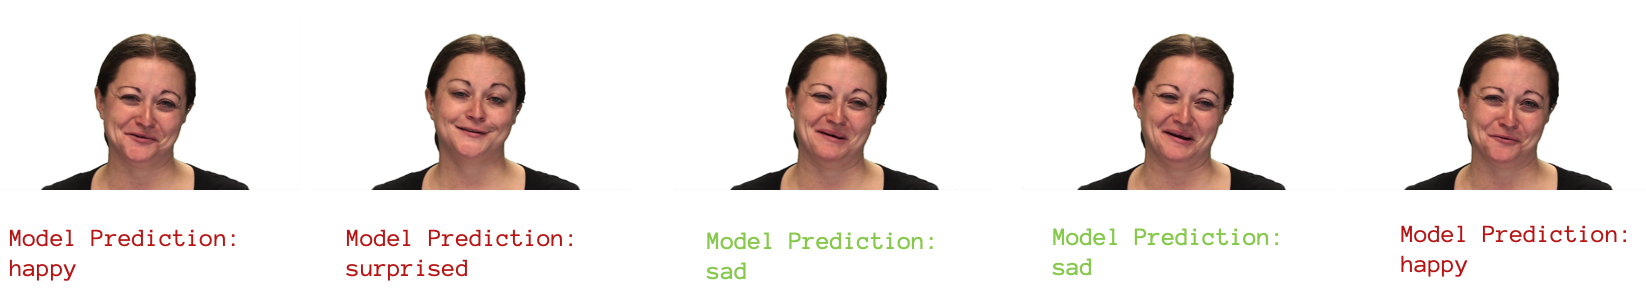
\includegraphics[width=0.8\textwidth]{res/modelex.png}
    \caption{An example of a model mislabeling a speaking subject talking while expressing a \texttt{sad} emotion \cite{livingstone2018ryerson}. Ideally, all frames, or the collection of frames, would be correctly categorized as \texttt{sad}.}
    \label{fig:mislabel}
\end{figure}